\chapter{Introduction}
Traditionally, hall mappers and stretched wire systems have been
used to measure solenoids at CERN. Recently, an alternative method
has been introduced. Using printed circuit board as fluxmeters,
induction coils can be very precisely engineered in desired shapes
and and sizes. Offering a large number of turns in a small area
compared to traditionally designed measurement coils.
\cite{petrone_induction-coil_2022}

A measurement system using such a fluxmeter has been proposed for
the new electron cooler being built for the AD experiment at CERN.
This system now needs to be evaluated, and redesigned for the
particular needs of the AD cooler.


\section{Principles of Electron Cooling}
As a particle beam is traveling through a particle accelerator, the spread
of the particles must be kept to a minimum. All the particles should have
nearly the same momentum, low positional spread and as little transverse
velocity as possible. This minimizes the amount of particles that are lost
in the path to their destination.

Electron coolers are used to decrease the transversal momentum and
spread for anti protons
or negative ion beams. The cooler is mounted along the beam path, as seen in
figure \ref{fig:ecooler}.

\begin{figure}[!h]
    \centering
    \includegraphics[width=0.8\textwidth]{figs/ecooler}
    \caption{An electron cooler. 3D model courtesy of CERN, EN-MME group.}
    \label{fig:ecooler}
\end{figure}

Electrons are shot from an electron gun into the gun solenoid. In the
first toroid section they are "kicked" into the beam path. The beam particles
will now collide with the electrons. Because both the beam particles and
the electrons are negatively charged, the momentum will be
transferred to the electrons through Coulomb interactions. This in effect
reduces the temperature of the beam. The now hot electrons are
then taken out of the beam path in the second toroid, into an electron collector.
This repeats for several turns, until the particle beam is sufficiently cooled.

The magnets in the cooler are weak, in the order of tens of milliteslas.
They affect the path of the electrons by a large degree, but
not the path of the much heavier beam particles.

\begin{figure}[!h]
    \centering
    \centering
    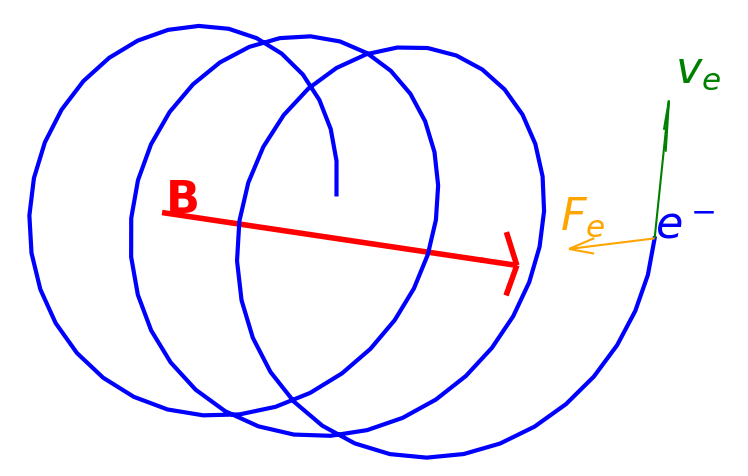
\includegraphics[width=0.6\linewidth]{figs/epath}
    \caption{An electron moving forwards in a solenoidal magnetic field,
        with its velocity $v_e$ and Lorentz force $F_e$. Solenoidal field axis $B$ in red.}
    \label{fig:epath}
\end{figure}

Because the magnets in the cooler are solenoids, the electrons will follow a
spinning path through the cooler according to the Lorentz Force, as seen in
figure \ref{fig:epath}. The higher the transversal momentum of the electrons,
the greater the Lorentz force keeping them inside the specified path.
Great care is taken to ensure that the electron cloud has the desired
beam velocity. Any beam particles that deviates from the desired
velocity, both axially and transversally, will transfer a higher amount
of momentum to the electrons. Beam particles that already have the desired
velocity and low transversal momentum, will see the electrons as stationary,
and thus go through the cooler relatively unchanged. \cite{d_functional_2023-fs}
The functional operation
of the electron cooler is very dependent on the field quality in the
main drift solenoid. Any non solenoidal field components will throw
the electrons off their intended path, thus necessitating high quality
magnetic measurements of the cooler.
\subsection{The new AD cooler}
The path of the solenoid windings, it's placement and manufacturing
irregularities all contribute to non solenoidal field components.
Additionally, the fringe fields of the surrounding magnets in the
toroidal sections also add unwanted field harmonics. Because of this,
a way of compensating for these components are needed.

\newpage
\begin{wrapfigure}{l}{0.4\textwidth}
    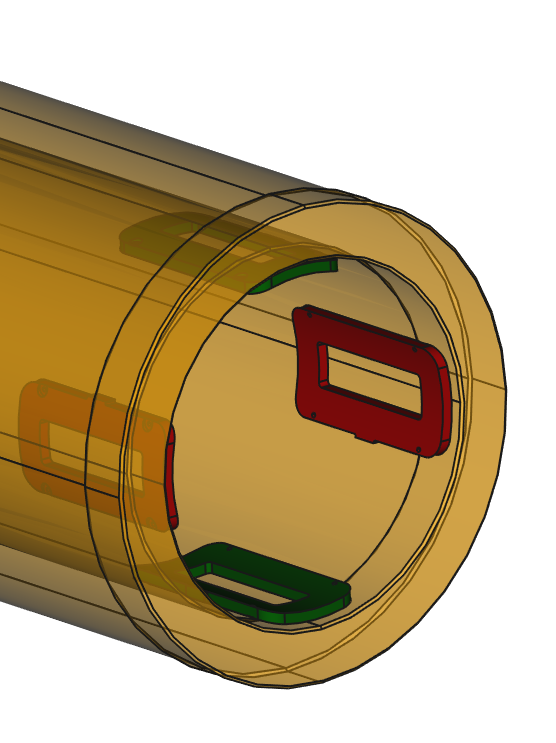
\includegraphics[width=0.9\linewidth]{figs/dipolecorrectors}
    \caption{Dipole correctors (red and green) at the end of a
        solenoid.}
    \label{fig:dipolecorrectors}
\end{wrapfigure}

The new AD cooler is still in its design phase. In the first pass,
the main drift solenoid was made up of several smaller "pancake"
solenoids, as seen in figure \ref{fig:ecooler}. These pancakes could
be individually tilted along their yaw and pitch axes, as well as moved.
The alignment of this pancake array would be done by measuring each
pancake at different tilt/swing angles, to get a field transfer function
with respect to the pancake orientation. These transfer functions would
then be linearly combined, to get the most optimal geometric configuration
for each coil.

The most recent design, at the time of writing instead makes use of
one long drift solenoid, along with several dipole correctors along the
length of the magnet, as illustrated in figure \ref{fig:dipolecorrectors}.

\section{The Measurement System}
The measurement system consists of a PCB fluxmeter with 21 coils printed on it.
This PCB is then moved laterally through the magnet aperture.
The coils then intercept the magnetic flux inside the aperture,
which can be read as a voltage. By keeping track of the fluxmeter's
geometric position, a field map with respect to the aperture length
can be acquired for each coil.

\begin{figure}[!h]
    \centering
    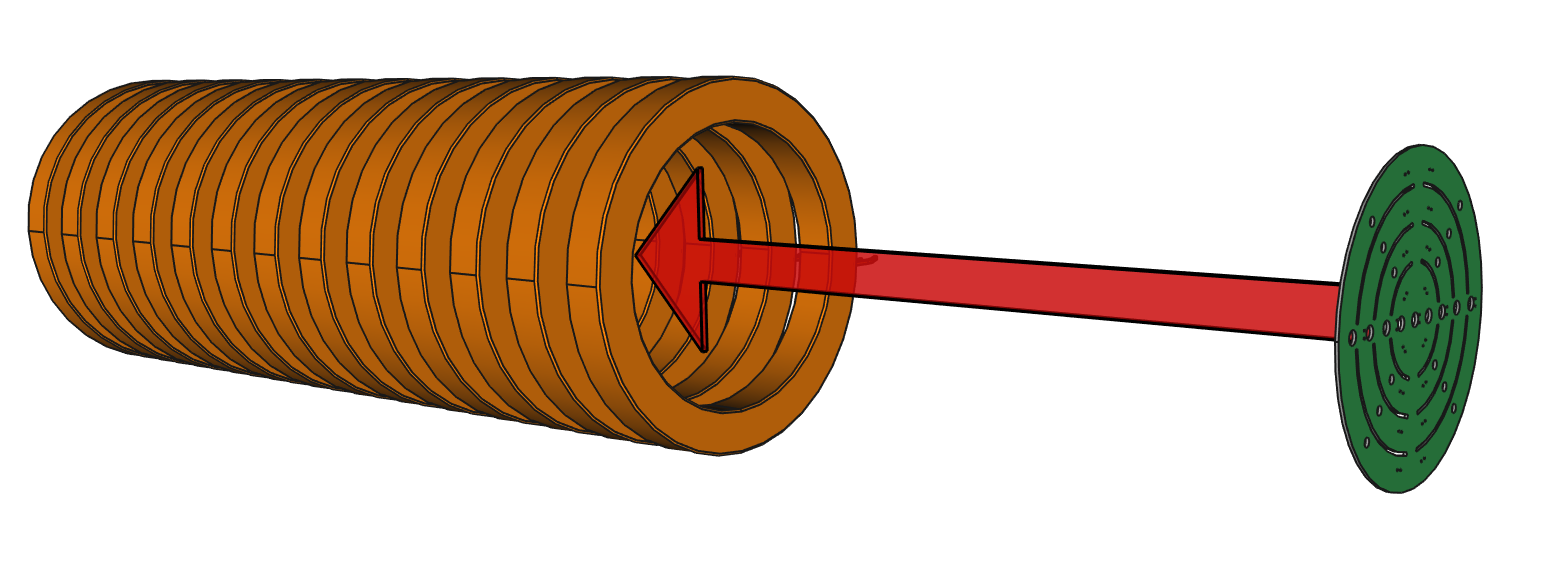
\includegraphics[width=0.6\textwidth]{figs/pcbpath}
    \caption{The fluxmeter entering the magnet aperture.}
    \label{fig:pcbpath}
\end{figure}

\section{Project Purpose and Goal}
The stringent requirements on the field of the AD cooler means the
magnetic measurements must be of high quality. Given that this is
a relatively new measurement methodology, meterological characterization
must be done to evaluate the system. The first design of the AD cooler
would have required measurements of field with respect to the tilt/swing
angle of each individual pancake solenoid. Even though this design was
later discarded, the question of mapping the field measurements to
the misalignment of the solenoid was still deemed to be of interest.
One goal is thus to find out if the pitch and yaw of a solenoid magnet
can be estimated using the magnetic measurements of the fluxmeter.
With such an approach, a solenoid could then be aligned correctly
to the beam aperture with iterative measurements and calibrations.
In the same vein, the minimum detectable angle is of course of interest,
as well as the sensitivity and accuracy of the field measurements.

The initial proposal for measuring the relative pitch/yaw was to
use two coils on opposite sides of the axis, as in figure \ref{fig:coil-dz}.

\begin{figure}[!h]
    \centering
    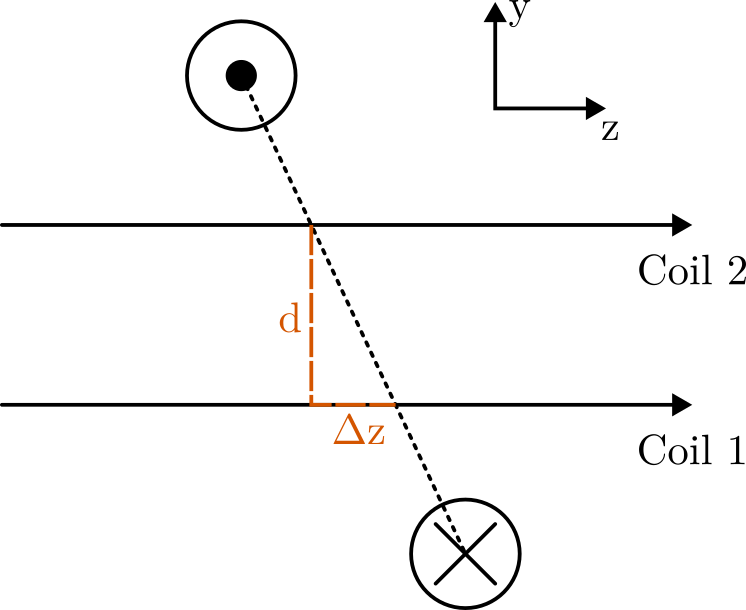
\includegraphics[width=0.6\textwidth]{figs/coil-dz}
    \caption{Two coils measuring the $\vb{B}$ field at different offsets
        from the axis.}
    \label{fig:coil-dz}
\end{figure}

The field in a solenoid is strongest in the middle. As coil 1
and 2 moves through the aperture, they will hit the peak field at different
times. Through some simple trigonometry, the relative tilt between the
solenoid and fluxmeter axis can then be estimated from the distance between
the peaks $\Delta z$ and the distance between the coils $d$.
\begin{equation}
    \theta = \arctan \left( \frac{d}{\Delta z} \right)
\end{equation}

Where $\theta$ is the relative tilt angle.
This model was not tested however, and thus needed to be verified.


Some work has already been done on the system, for instance on measuring
the longitudinal and transversal field components, as well as estimating
the field axis. \cite{petrone_induction-coil_2022}